\documentclass[10pt,landscape,a4paper]{article}
\usepackage[utf8]{inputenc}
\usepackage[ngerman]{babel}
\usepackage{tikz}
\usetikzlibrary{shapes,positioning,arrows,fit,calc,graphs,graphs.standard}
\usepackage[nosf]{kpfonts}
\usepackage[t1]{sourcesanspro}
%\usepackage[lf]{MyriadPro}
%\usepackage[lf,minionint]{MinionPro}
\usepackage{multicol}
\usepackage{wrapfig}
\usepackage[top=0mm,bottom=1mm,left=0mm,right=1mm]{geometry}
\usepackage[framemethod=tikz]{mdframed}
\usepackage{microtype}

\DeclareMathOperator*{\argmin}{arg\,min}
\DeclareMathOperator*{\argmax}{arg\,max}
\newcommand{\vek}[1]{\mathbf{#1}}
\newcommand*{\vertbar}{\rule[-1ex]{0.5pt}{2.5ex}}
\newcommand*{\horzbar}{\rule[.5ex]{2.5ex}{0.5pt}}


\let\bar\overline

\definecolor{myblue}{cmyk}{1,.72,0,.38}

\def\firstcircle{(0,0) circle (1.5cm)}
\def\secondcircle{(0:2cm) circle (1.5cm)}

\colorlet{circle edge}{myblue}
\colorlet{circle area}{myblue!5}

\tikzset{filled/.style={fill=circle area, draw=circle edge, thick},
    outline/.style={draw=circle edge, thick}}

\pgfdeclarelayer{background}
\pgfsetlayers{background,main}

\everymath\expandafter{\the\everymath \color{myblue}}
\everydisplay\expandafter{\the\everydisplay \color{myblue}}

\renewcommand{\baselinestretch}{.8}
\pagestyle{empty}

\global\mdfdefinestyle{header}{%
linecolor=gray,linewidth=1pt,%
leftmargin=0mm,rightmargin=0mm,skipbelow=0mm,skipabove=0mm,
}

\newcommand{\header}{
\begin{mdframed}[style=header]
\footnotesize
\sffamily
COMP 652 - Machine Learning\\
by~Carlos G. Oliver,~page~\thepage~of~2
\end{mdframed}
}

\makeatletter
\renewcommand{\section}{\@startsection{section}{1}{0mm}%
                                {.2ex}%
                                {.2ex}%x
                                {\color{myblue}\sffamily\small\bfseries}}
\renewcommand{\subsection}{\@startsection{subsection}{1}{0mm}%
                                {.2ex}%
                                {.2ex}%x
                                {\sffamily\bfseries}}



\def\multi@column@out{%
   \ifnum\outputpenalty <-\@M
   \speci@ls \else
   \ifvoid\colbreak@box\else
     \mult@info\@ne{Re-adding forced
               break(s) for splitting}%
     \setbox\@cclv\vbox{%
        \unvbox\colbreak@box
        \penalty-\@Mv\unvbox\@cclv}%
   \fi
   \splittopskip\topskip
   \splitmaxdepth\maxdepth
   \dimen@\@colroom
   \divide\skip\footins\col@number
   \ifvoid\footins \else
      \leave@mult@footins
   \fi
   \let\ifshr@kingsaved\ifshr@king
   \ifvbox \@kludgeins
     \advance \dimen@ -\ht\@kludgeins
     \ifdim \wd\@kludgeins>\z@
        \shr@nkingtrue
     \fi
   \fi
   \process@cols\mult@gfirstbox{%
%%%%% START CHANGE
\ifnum\count@=\numexpr\mult@rightbox+2\relax
          \setbox\count@\vsplit\@cclv to \dimexpr \dimen@-1cm\relax
\setbox\count@\vbox to \dimen@{\vbox to 1cm{\header}\unvbox\count@\vss}%
\else
      \setbox\count@\vsplit\@cclv to \dimen@
\fi
%%%%% END CHANGE
            \set@keptmarks
            \setbox\count@
                 \vbox to\dimen@
                  {\unvbox\count@
                   \remove@discardable@items
                   \ifshr@nking\vfill\fi}%
           }%
   \setbox\mult@rightbox
       \vsplit\@cclv to\dimen@
   \set@keptmarks
   \setbox\mult@rightbox\vbox to\dimen@
          {\unvbox\mult@rightbox
           \remove@discardable@items
           \ifshr@nking\vfill\fi}%
   \let\ifshr@king\ifshr@kingsaved
   \ifvoid\@cclv \else
       \unvbox\@cclv
       \ifnum\outputpenalty=\@M
       \else
          \penalty\outputpenalty
       \fi
       \ifvoid\footins\else
         \PackageWarning{multicol}%
          {I moved some lines to
           the next page.\MessageBreak
           Footnotes on page
           \thepage\space might be wrong}%
       \fi
       \ifnum \c@tracingmulticols>\thr@@
                    \hrule\allowbreak \fi
   \fi
   \ifx\@empty\kept@firstmark
      \let\firstmark\kept@topmark
      \let\botmark\kept@topmark
   \else
      \let\firstmark\kept@firstmark
      \let\botmark\kept@botmark
   \fi
   \let\topmark\kept@topmark
   \mult@info\tw@
        {Use kept top mark:\MessageBreak
          \meaning\kept@topmark
         \MessageBreak
         Use kept first mark:\MessageBreak
          \meaning\kept@firstmark
        \MessageBreak
         Use kept bot mark:\MessageBreak
          \meaning\kept@botmark
        \MessageBreak
         Produce first mark:\MessageBreak
          \meaning\firstmark
        \MessageBreak
        Produce bot mark:\MessageBreak
          \meaning\botmark
         \@gobbletwo}%
   \setbox\@cclv\vbox{\unvbox\partial@page
                      \page@sofar}%
   \@makecol\@outputpage
     \global\let\kept@topmark\botmark
     \global\let\kept@firstmark\@empty
     \global\let\kept@botmark\@empty
     \mult@info\tw@
        {(Re)Init top mark:\MessageBreak
         \meaning\kept@topmark
         \@gobbletwo}%
   \global\@colroom\@colht
   \global \@mparbottom \z@
   \process@deferreds
   \@whilesw\if@fcolmade\fi{\@outputpage
      \global\@colroom\@colht
      \process@deferreds}%
   \mult@info\@ne
     {Colroom:\MessageBreak
      \the\@colht\space
              after float space removed
              = \the\@colroom \@gobble}%
    \set@mult@vsize \global
  \fi}

\makeatother
\setlength{\parindent}{0pt}

\begin{document}
\small
\begin{multicols*}{5}

%%%% MATH %%%%%%

\section{Math}
{\bf Bayes rule: } $P(A \vert B) = \frac{P(A, B)}{P(B)} = \frac{P(B \vert A) P(A)}{P(B)}$\\
{\bf Chain rule: } $P(A_n, \ldots , A_1)  = \mathrm P(A_n | A_{n-1}, \ldots , A_1) \cdot\mathrm P( A_{n-1}, \ldots , A_1)$\\
{\bf Joint: } $\mathrm  P\left(\bigcap_{k=1}^n A_k\right)  = \prod_{k=1}^n  \mathrm P\left(A_k \,\Bigg|\, \bigcap_{j=1}^{k-1} A_j\right)$\\
{\bf Posterior:} unobserved $\theta$, observed $x$: $p(\theta \vert x) = \frac{p(x \vert \theta)p(\theta)}{p(x)}$\\
{\bf Prior:} prior belief in dist. of $\theta$: $p(\theta)$\\
{\bf Likelihood:} prob of observed given parameters: $p(x \vert \theta)$\\
{\bf MAP:} $h_{MAP} = \argmax_{h\in H} P(h \vert D) = \argmax_{h\in H} P(D \vert h) P(h)$\\ 
{\bf Lagrange: } $L(\vek{x}, \lambda) = f(\vek{x}) + \lambda g(\vek{x})$
Set constraint $g(\vek{x})$ to zero and add multiplier. \\
$$\vek{xy^T} = \begin{bmatrix}
           x_{1} \\
           \vdots \\
           x_{m}
         \end{bmatrix}      
         \begin{bmatrix}
           x_{1}\hdots x_{n}
         \end{bmatrix} = \begin{bmatrix}
         x_1 y_1 & \hdots & x_1 y_n \\
         \vdots & \ddots  & \vdots \\
          x_m y_1 & \hdots & x_m y_n \\
         \end{bmatrix}
         $$
{\bf Matrix-vector product: } $ \vek{Ax} = \begin{bmatrix}
 	a_1^T\vek{x}\\
	\vdots \\
	a_m^T\vek{x}
	\end{bmatrix}
$

{\bf Matrix mult': } $ (\mathbf{A}\mathbf{B})_{ij} = \sum_{k=1}^m A_{ik}B_{kj}\,$

$$ \vek{AB} =  \begin{bmatrix}
         a_1^Tb_1&  a_1^T b_2 & \hdots & a_1^T b_p \\
         \vdots & \vdots  & \ddots  & \vdots \\
          a_m^T b_1 & a_m^T b_2 & \hdots & a_m^T b_n \\
         \end{bmatrix}
$$

$(n \times p)(p \times m) = n \times p$


\section{todo}
\begin{itemize}
\item Marginals
\item Eigendecomposition
\item $\sin(x)^{'} = \cos{x}$
\item $\cos(x)^{'} = -\sin{x}$
\item 
\item $(AB)^{T} = B^{T}A$
\item $\log_{b}(x^{y}) = y \log_{b}(x)$
\item Uniform distribution: $P_{\theta_1, \theta_2}(x) = \frac{1}{\theta_2 - \theta_1}$
\item $AA^{-1} = A^{-1}A = I$ for square matrices.
\item $F'(x) = f'(g(x)) g'(x)$
\item $(f\cdot g)'=f'\cdot g+f\cdot g' \,\!$
\item Log properties
\item Convexity
\item $\vert \vert \vek{x} \vert \vert_{d} = \sum_{i} x_{i}^{d}$
\item Polynomial multiplication
\item Matrix transpose and inverse tproperties
\item Gradient vs partial derivative
\item $\sigma(x)^{'} = \sigma(x)(1-\sigma(x))$
\item $\mathrm{E}\Big[\big(y - \hat{f}(x)\big)^2\Big] = \mathrm{E}\big[\hat{f}(x) - f(x)\big]^2 + \mathrm{E}[\hat{f}(x)^2] - \mathrm{E}[\hat{f}(x)]^2 + \epsilon^2$
\end{itemize}


%%%% EARLY STUFF %%%

\section{Regression}
\subsection{L2 regularization}
Weights do not reach zero. Faster.
$$J_w = \frac{1}{2}(\Phi\vek{w} - \vek{y})^T(\Phi \vek{w} - \vek{y}) + \frac{\lambda}{2}\vek{w}^T\vek{w}$$
$$\vek{w} = (\Phi^T\Phi + \lambda \vek{I})^{-1}\Phi^Ty$$
\subsection{L1 regularization}
Some weights set to zero. More expensive. 
\subsection{Gradient Descent}
$\vek{w} \leftarrow \vek{w} - \alpha \nabla \log L(\vek{w})$
$\vek{w} \leftarrow \vek{w} - \alpha \nabla \log J(\vek{w})$

\subsection{Bayesian regularization}


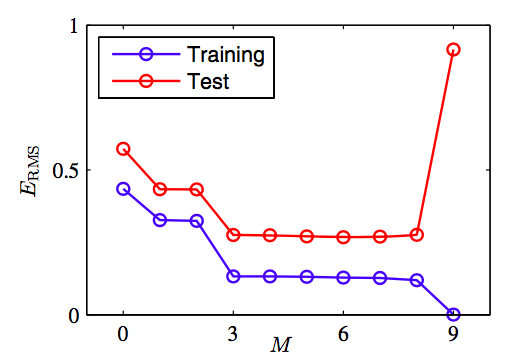
\includegraphics[width=\linewidth]{error.png}

\section{Kernels}
$k(\vek{x}, \vek{z}) = \phi(\vek{x}) \cdot \phi(\vek{z})$
{\bf Mercer theorem:} $K(\vek{x}, \vek{z})$ is kernel iff Gram matrix $\vek{K}$ symmetric and positive semidefinite: $\vek{K_{ij}} = \vek{K_{ji}}$ and $\vek{z}^{T}\vek{K}\vek{z} \geq 0$
$\vek{K} = \Phi\Phi^T$ where $\vek{K_{nm}} = \phi(\vek{x_n})^T\phi(\vek{x_m}) = k(\vek{x_n}, \vek{x_m})$ Gram matrix size of input.


\begin{itemize}
\item Kernel properties
\item Proving kernels
\end{itemize}

\section{SVM}
Minimize absolute error. More robust to outliers. Max margin is convex optimization.
$$h_{\vek{w}}(\vek{x}) = \text{sign}(\sum_{i=1}^m \alpha_{i}y_{i}(\vek{x_{i}}\vek{x}) + \vek{w_0})$$

$\alpha_{i} > 0$ only for support vectors. Soft error SVM: $0 < \zeta \leq 1$ if inside margin. $\zeta > 1$ if misclassified. Total errors: $C \sum_{i} \zeta$. Large $C$ higher variance.

\section{EM/Active Learning/Missing Data}

\end{multicols*}
\end{document}